\section{Tracking Block Design}
\label{sec:tracking}

The tracking block uses camera inputs to calculate hand positions, which are
then sent to the gameplay block. Four modules 
comprise the block: the camera module, the frame buffer, the center of mass
module, and the position module. Information flow between these modules is shown
in figure \ref{fig:tracking}.

\begin{figure}
\centering
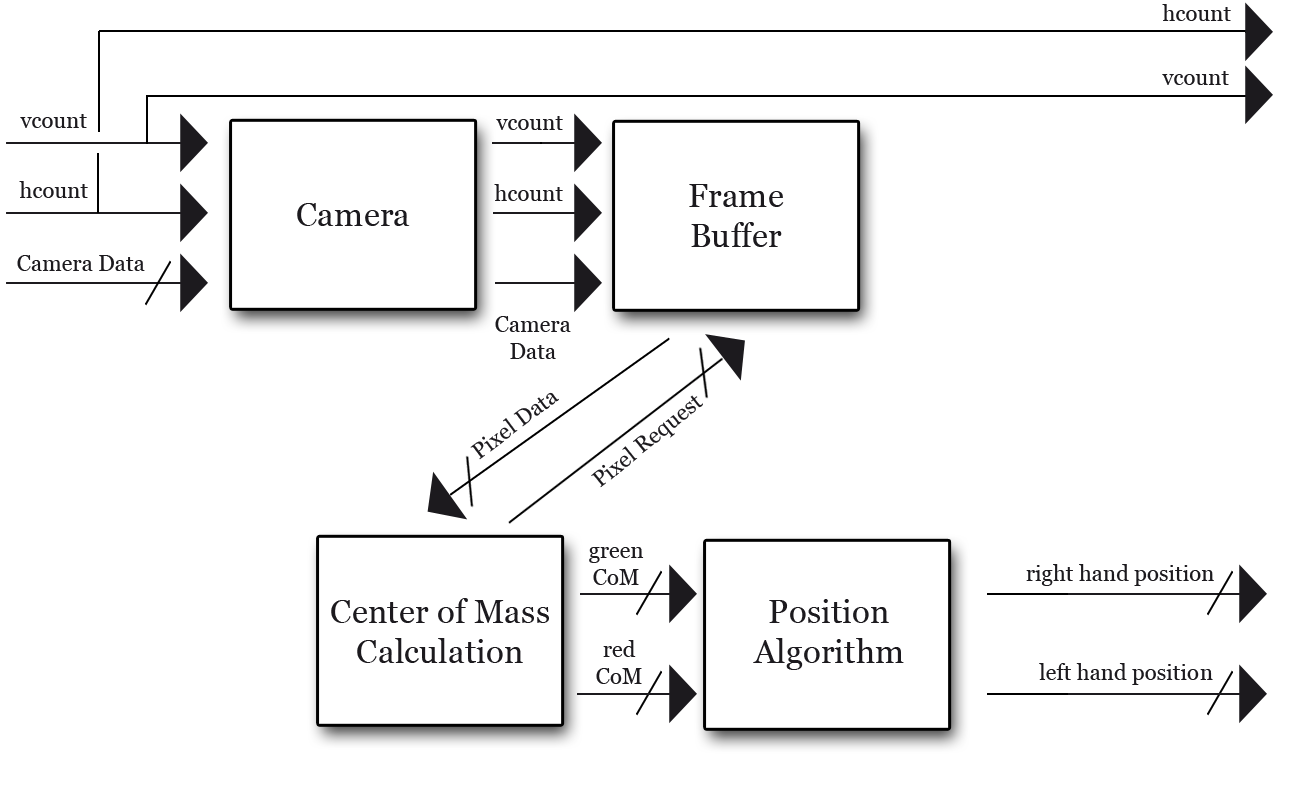
\includegraphics[scale=1]{img/tracking.png}
\caption{The tracking system has four primary steps. First, information is
processed from the raw camera input. Second, frames are stored for later use.
Third, center of mass information is calculated for each glove. Finally, a
smoothing function using past position information to prevents errors and noise.
The result is accurate information describing the position of the player's
hands in the real world.}
\label{fig:tracking}
\end{figure}

\subsection{Camera Module}

The camera module has the responsibility of taking in and processing the
information from the NTSC camera.

The NTSC camera output is connected to the 6.111 lab FPGA board. A set of
modules provided by the 6.111 staff processes the input signal and extracts
YCrCb color information, horizontal sync, vertical sync, and field data. This
data is then passed through a YCrCb to RGB converter and on into the
nts\_to\_zbt module, which prepares the information for
storage in the zbt ram.

Color is downsampled to eighteen bits, six each for red, green, and blue. This
allows the storage of two pixels in each thirty-six-bit memory slot. Pixels are
stored in an address indexed by their concatenated y and x coordinates on the
screen, dropping the last bit because two pixels share each memory slot.
ntsc\_to\_zbt counts the x and y coordinate of the incoming pixel data and
caluclates a memory address based on this information. In doing this
calculation, it takes into account the fact that a mirrored screen gives a more
intuitive interface for a user and thereby uses $719-x$ for the x coordinate
of the pixel. This mirroring assures that a leftward motion of the user's hand
is shown as a leftward motion on the screen, rather that rightward.  This module
also concatenates the color data for two consecutive pixels, producing the data
to be stored in a single memory slot. Finally, ntsc\_to\_zbt syncronizes this
information with the $65Mhz$ system clock where it was previously syncronized
with the camera input clock.

\subsection{Frame Buffer}

The decision was made to use only a single frame buffer for both storage and
retrieval. The simplicity of the calculation involving individual pixels made it
clear that a two-frame buffer would not be necessary.  because of this, data
from the ntsc\_to\_zbt module is passed directly to the 6.111-provided zbt\_6111
module, which stores the provided information in the provided address of zbt
memory.

The same zbt\_6111 module handles output from memory to the center-of-mass
module. The 6.111-provided vram\_display module calculates
the address of the relevant pixel using the xvga module's control signals and
sends that to zbt\_6111. Read-write is chosen based on the last bit of the
current camera hcount.

\subsection{Center of Mass Module}

The center of mass module calculates the center of mass of certain shades of red
and green in each frame, outputting the x and y coordinates of each.

Input from the zbt\_6111 read commands is fed into each of two center of mass
(centerOfMass in the verilog files) modules along with the value of each of the
8 6.111 lab board switches and two button inputs, one reset button and one set
button.

The hcount and vcount information is first checked to see if the current pixel
is valid. Any pixel outside of the 720 by 480 camera input area is discarded as
unnecessary. Following this check, the pixel is compared to a certain set of
criteria and, if it fits them, deemed part of the glove. These criteria come in
three parts. First a color selection signal indicates whether we are tracking a
red, green, or blue (the "primary color" object). Next, a minimum value is set
for the primary color. Any pixel for which the primary color is below the
minimum is ignored. Finally, a minimum difference is set for each of the two
remaining "secondary" colors is defined. This minimum difference requires that
the value of each of the other colors in the pixel be at least a certain amount
below the value for the primary color. If either secondary color is larger than
$primary\_color - minimum\_difference$ the pixel is ignored. What remains are a
set of pixels that match an expected color profile.

Setting the right color profile is the most difficult part of the problem.
Because the lighting within the scene can vary depending on the user's hand
position and angle, only very specific settings allow for good tracking across
all possible user hand positions. Additionally, every time the system is used
the lighting will be slightly different. The only simple way to overcome this
was to provide a calibration mode allowing the user to determine the best
settings for a given scene and lighting.

The eight switch and two button inputs provide this phenomenally helpful
configuration control. Two screens are available to the user along with the game
screen. Button $0$ toggles between them. One allows for configuration of the red
glove tracking and the other for configuration of the green glove tracking. When
on these screens the user may press button $2$ in order to "reset" the
tracking and require the system to use the inputs of switches 0 through 3 as the
minimum difference value and switches 4 through 7 for the minimum primary color
value. These screens highlight all pixels interpreted by th module as part of
the glove in green or red, depending on the glove in question, and show the
center of mass using one vertical and one horizontal line. This information and
experimentation allow the user to determine the best possible settings for
tracking each glove. Hitting button $1$ sets the current switch values as the
tracking settings.

All of this functionality is implemented inside the center of mass module,
including detection of the button signal edges, storage of the set values, and
selecting between the set values and the switch values depending on the system
state. A set of four configurations, each of higher accuracy than the last, can
be seen in figure \ref{fig:config}.

\begin{figure}[h]
\centering
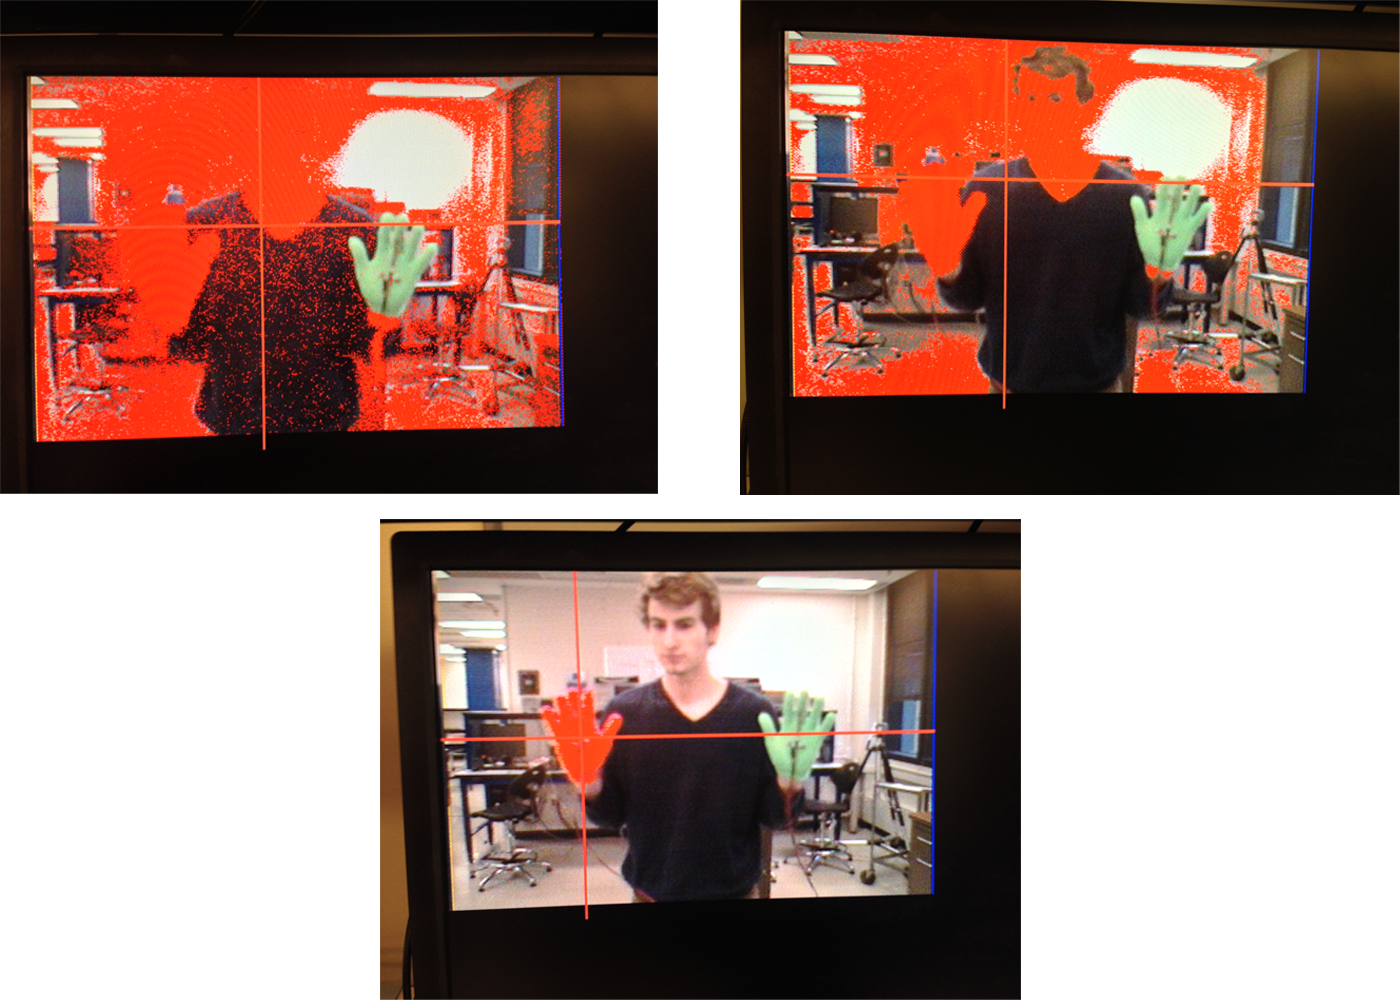
\includegraphics[width=6.5in]{img/config.png}
\caption{Configuration involves the modification of two variables, the minimum
primary color value and the minimum color difference, to define which pixels are
part of the glove. Three stages of configuration are shown, demonstrating the
importance of this configuration step.}
\label{fig:config}
\end{figure}

Two more steps are necessary for accurate tracking. First, weighting based on
adjacent pixels biases the center of mass toward large blocks of color instead
of isolated pixels that could be the result of random noise in the video camera.
This is done by pushing pixels through three registers. Each pixel is considered
when it reaches the second register and weighted based not only on its own color
but also on the color of the pixel immediately before and after it. As it is
implemented, this has an odd effect of relating the last pixel in each row with
the first two of the next. Fixing this would be good but is not strictly
necessary from a functionality prospective, considering how unlikely it is for
any two specific pixels to encounter unlikely noise on the same frame.

Pixels with no adjacent pixels of the correct color are weighted with a $1$,
pixels with one adjacent pixel of the correct color are weighted with a $2$, and
pixels with both adjacent pixels of the correct color are weighted with a $4$.

The final step is to accumulate three weighted sums, one of the x coordinates of
all matching pixels, one of the y coordinates, and one of the number of pixels
matching. When both hcount and vcount hit zero, these values are fed into
dividers and reset to zero before the first pixel of the next frame is
considered. The divider outputs are the x and y centers of the color in
question.

Each center of mass module considers only one color at a time. Two are used, one
for green and one for red.

\subsection{Position Module}

The position module takes as input the center of mass position output and
further refines it. Even after the careful work of the center of mass module
random noise still resulted in erratic motion of the user hand position on
screen. To fix this, the last four center of mass positions are passed through
registers and the position of the user's hands in each frame is defined by the
average of those four values. This implements a simple low-pass filter and
removes any high-frequency noise caused by random glitches. The output of this
module is the stabilized hand position. Two such modules are used, one for the
green hand and one for the red.

